\documentclass[11pt,a4paper]{article}

\usepackage[T1]{fontenc}
\usepackage[utf8]{inputenc}
\usepackage[british]{babel}
\usepackage[left=0mm,right=0mm,top=0mm,bottom=0mm]{geometry}
\usepackage[stretch=25,shrink=25,tracking=true,letterspace=30]{microtype}
\usepackage{graphicx}
\usepackage{xcolor}
\usepackage{marvosym}
\usepackage{enumitem}
\setlist{parsep=0pt,topsep=0pt,partopsep=1pt,itemsep=1pt,leftmargin=6mm}
\usepackage{FiraSans}
\renewcommand{\familydefault}{\sfdefault}
\definecolor{cvblue}{HTML}{304263}

% --- Macros perso ------------------------------------------------------------
\newcommand{\dates}[1]{\hfill\mbox{\textbf{#1}}}
\newcommand{\is}{\par\vskip.5ex plus .4ex}
\newcommand{\smaller}[1]{{\small$\diamond$\ #1}}
\newcommand{\headleft}[1]{\vspace*{3ex}\textsc{\textbf{#1}}\par%
    \vspace*{-1.5ex}\hrulefill\par\vspace*{0.7ex}}
\newcommand{\headright}[1]{\vspace*{2.5ex}\textsc{\Large\color{cvblue}#1}\par%
     \vspace*{-2ex}{\color{cvblue}\hrulefill}\par}

\usepackage[colorlinks=true,urlcolor=white,linkcolor=white]{hyperref}

% -----------------------------------------------------------------------------

\begin{document}
\setlength{\topskip}{0pt}\setlength{\parindent}{0pt}\setlength{\parskip}{0pt}
\setlength{\fboxsep}{0pt}\pagestyle{empty}\raggedbottom

% ============================================================================
%                               COLONNE GAUCHE
% ============================================================================
\begin{minipage}[t]{0.33\textwidth}
\colorbox{cvblue}{\begin{minipage}[t][5mm][t]{\textwidth}\null\hfill\null\end{minipage}}
\vspace{-.2ex}
\colorbox{cvblue!90}{\color{white}
\kern0.09\textwidth
\begin{minipage}[t][293mm][t]{0.82\textwidth}\raggedright
\vspace*{2.5ex}

% ---- Identité ---------------------------------------------------------------
\Large Pape \textbf{\textsc{FALL}} \normalsize

\null\hfill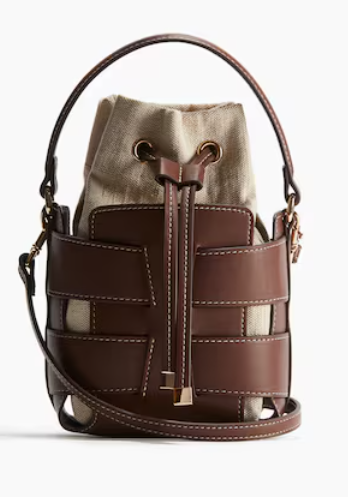
\includegraphics[width=0.65\textwidth]{ bc42cb00a46b4cb89cd6efe8aa85a343.png }\hfill\null

\vspace*{0.5ex}

% ---- Résumé -----------------------------------------------------------------
\headleft{Profile Summary}
Data Scientist passionné, diplômé de Sorbonne Université, avec une solide expérience de stages en data science et data analyse. Compétent dans l’ensemble du cycle de vie de la donnée : collecte, nettoyage, modélisation et visualisation. À l’aise avec Python, les bibliothèques ML/IA, SQL et les outils de BI. Curieux, rigoureux et doté d’un excellent sens business, je cherche à mettre mes compétences au service d’équipes data innovantes.

% ---- Contact ----------------------------------------------------------------
\headleft{Contact details}\small
\MVAt\ {\small papesalioufall2@gmail.com} \\[0.4ex]
\Mobilefone\ 0753481453 \\[0.5ex]
\Letter\ Paris, France
\normalsize

% ---- Infos perso ------------------------------------------------------------
\headleft{Personal information}
Citizenship: \textbf{Française} \\[0.5ex]
Family: \textbf{Célibataire} \\[0.5ex]
Languages: \textbf{Français (natif), Anglais (courant)}

% ---- Compétences ------------------------------------------------------------
\headleft{Skills}
\begin{itemize}
  \item Python
  \item R
  \item SQL
  \item Pandas, NumPy, Scikit-learn
  \item TensorFlow, Keras
  \item Machine Learning supervisé et non supervisé
  \item Deep Learning (CNN, RNN)
  \item Statistiques et modélisation
  \item Data Visualisation (Matplotlib, Seaborn, Power BI)
  \item Git \& Docker
  \item Cloud : AWS (S3, EC2, SageMaker)
\end{itemize}

\end{minipage}\kern 0.09\textwidth
}
\end{minipage}
% ============================================================================
%                               COLONNE DROITE
% ============================================================================
\hskip2.5em
\begin{minipage}[t]{0.56\textwidth}
\setlength{\parskip}{0.8ex}
\vspace{2ex}

% ------------------------ EXPÉRIENCE ----------------------------------------
\headright{Experience}
\textsc{Stagiaire data scientist} at \textit{Prepaya} (Paris, France)  \dates{2022-2024} \\
\smaller{Développé des modèles de prédiction de churn avec Scikit-learn (accuracy +12 \%).}\is
\smaller{Automatisé des pipelines ETL en Python, réduisant le temps de traitement de 40 \%.}\is
\smaller{Mis en place des dashboards Power BI pour le suivi des KPIs business.}\is
\smaller{Collaboré avec les équipes produit pour transformer les insights data en actions marketing.}\is

\textsc{Stagiaire data analyst} at \textit{Edf} (La Défense, France)  \dates{2023-2024} \\
\smaller{Analysé les données de consommation énergétique pour optimiser la prévision de la demande.}\is
\smaller{Créé des rapports interactifs sous Power BI pour 5 + équipes métiers.}\is
\smaller{Élaboré des scripts SQL avancés pour extraire et nettoyer 10 M + lignes de données.}\is
\smaller{Participé à des ateliers agiles, améliorant la communication entre data et business.}\is

% ------------------------ ÉDUCATION ----------------------------------------
\headright{Education}
\textsc{Master 2 Data science}. \textit{Sorbonne Université}. \dates{2022-2023} \\
\textsc{master 1 Data science}. \textit{Sorbonne Université}. \dates{2023-2024} \\

% ------------------------ CERTIFICATIONS ------------------------------------
\headright{Certifications}
\smaller{\textsc{IBM Data Science Professional Certificate}}, \textit{Coursera / IBM}. \dates{2023-05} \\
\smaller{\textsc{AWS Certified Cloud Practitioner}}, \textit{Amazon Web Services}. \dates{2024-02} \\

% ------------------------ HOBBIES -------------------------------------------
\headright{Hobbies}
\textit{Randonnée, photographie urbaine, échecs}

\end{minipage}

\end{document}